\section{Conception électronique}\label{sec:electronique}

\subsection{Protocole de communication}\label{subsec:protocole}

La station météo joue le rôle de concentrateur (\textit{hub}) de données entre
plusieurs systèmes hétérogènes. Le schéma de communication retenu est décrit
ci-dessous et illustré en figure~\ref{fig:protocole_comm}.

\paragraph{Réseau du bateau.} Les instruments du bateau (GPS, loch, girouette,
etc.) communiquent avec la station via le protocole \textit{NMEA 2000}, basé sur
le bus CAN (Controller Area Network). Ce standard est universellement adopté dans
le domaine maritime et permet d'interconnecter des équipements de marques
différentes sur un seul câble blindé à deux fils. Un transceiver CAN dédié assure
la conversion entre le bus et l'interface SPI de l'ESP32.

\paragraph{Sonde CTD.} La sonde CTD sous-marine est reliée à la station par câble.
Plusieurs interfaces ont été étudiées : Zigbee pour une liaison sans fil courte
portée, ou câblé en RS-485, Ethernet deux fils ou RS-232. Un port dédié est prévu
sur le PCB pour accommoder ces différentes options. Le module \textit{XIAO ESP32C6}
intégré au PCB gère la communication Zigbee.

\paragraph{Transmission vers l'ordinateur.} La station transmet les données
collectées vers un ordinateur portable à bord via Wi-Fi, permettant la
visualisation et l'enregistrement en temps réel sans liaison filaire.

\begin{figure}[H]
  \centering
  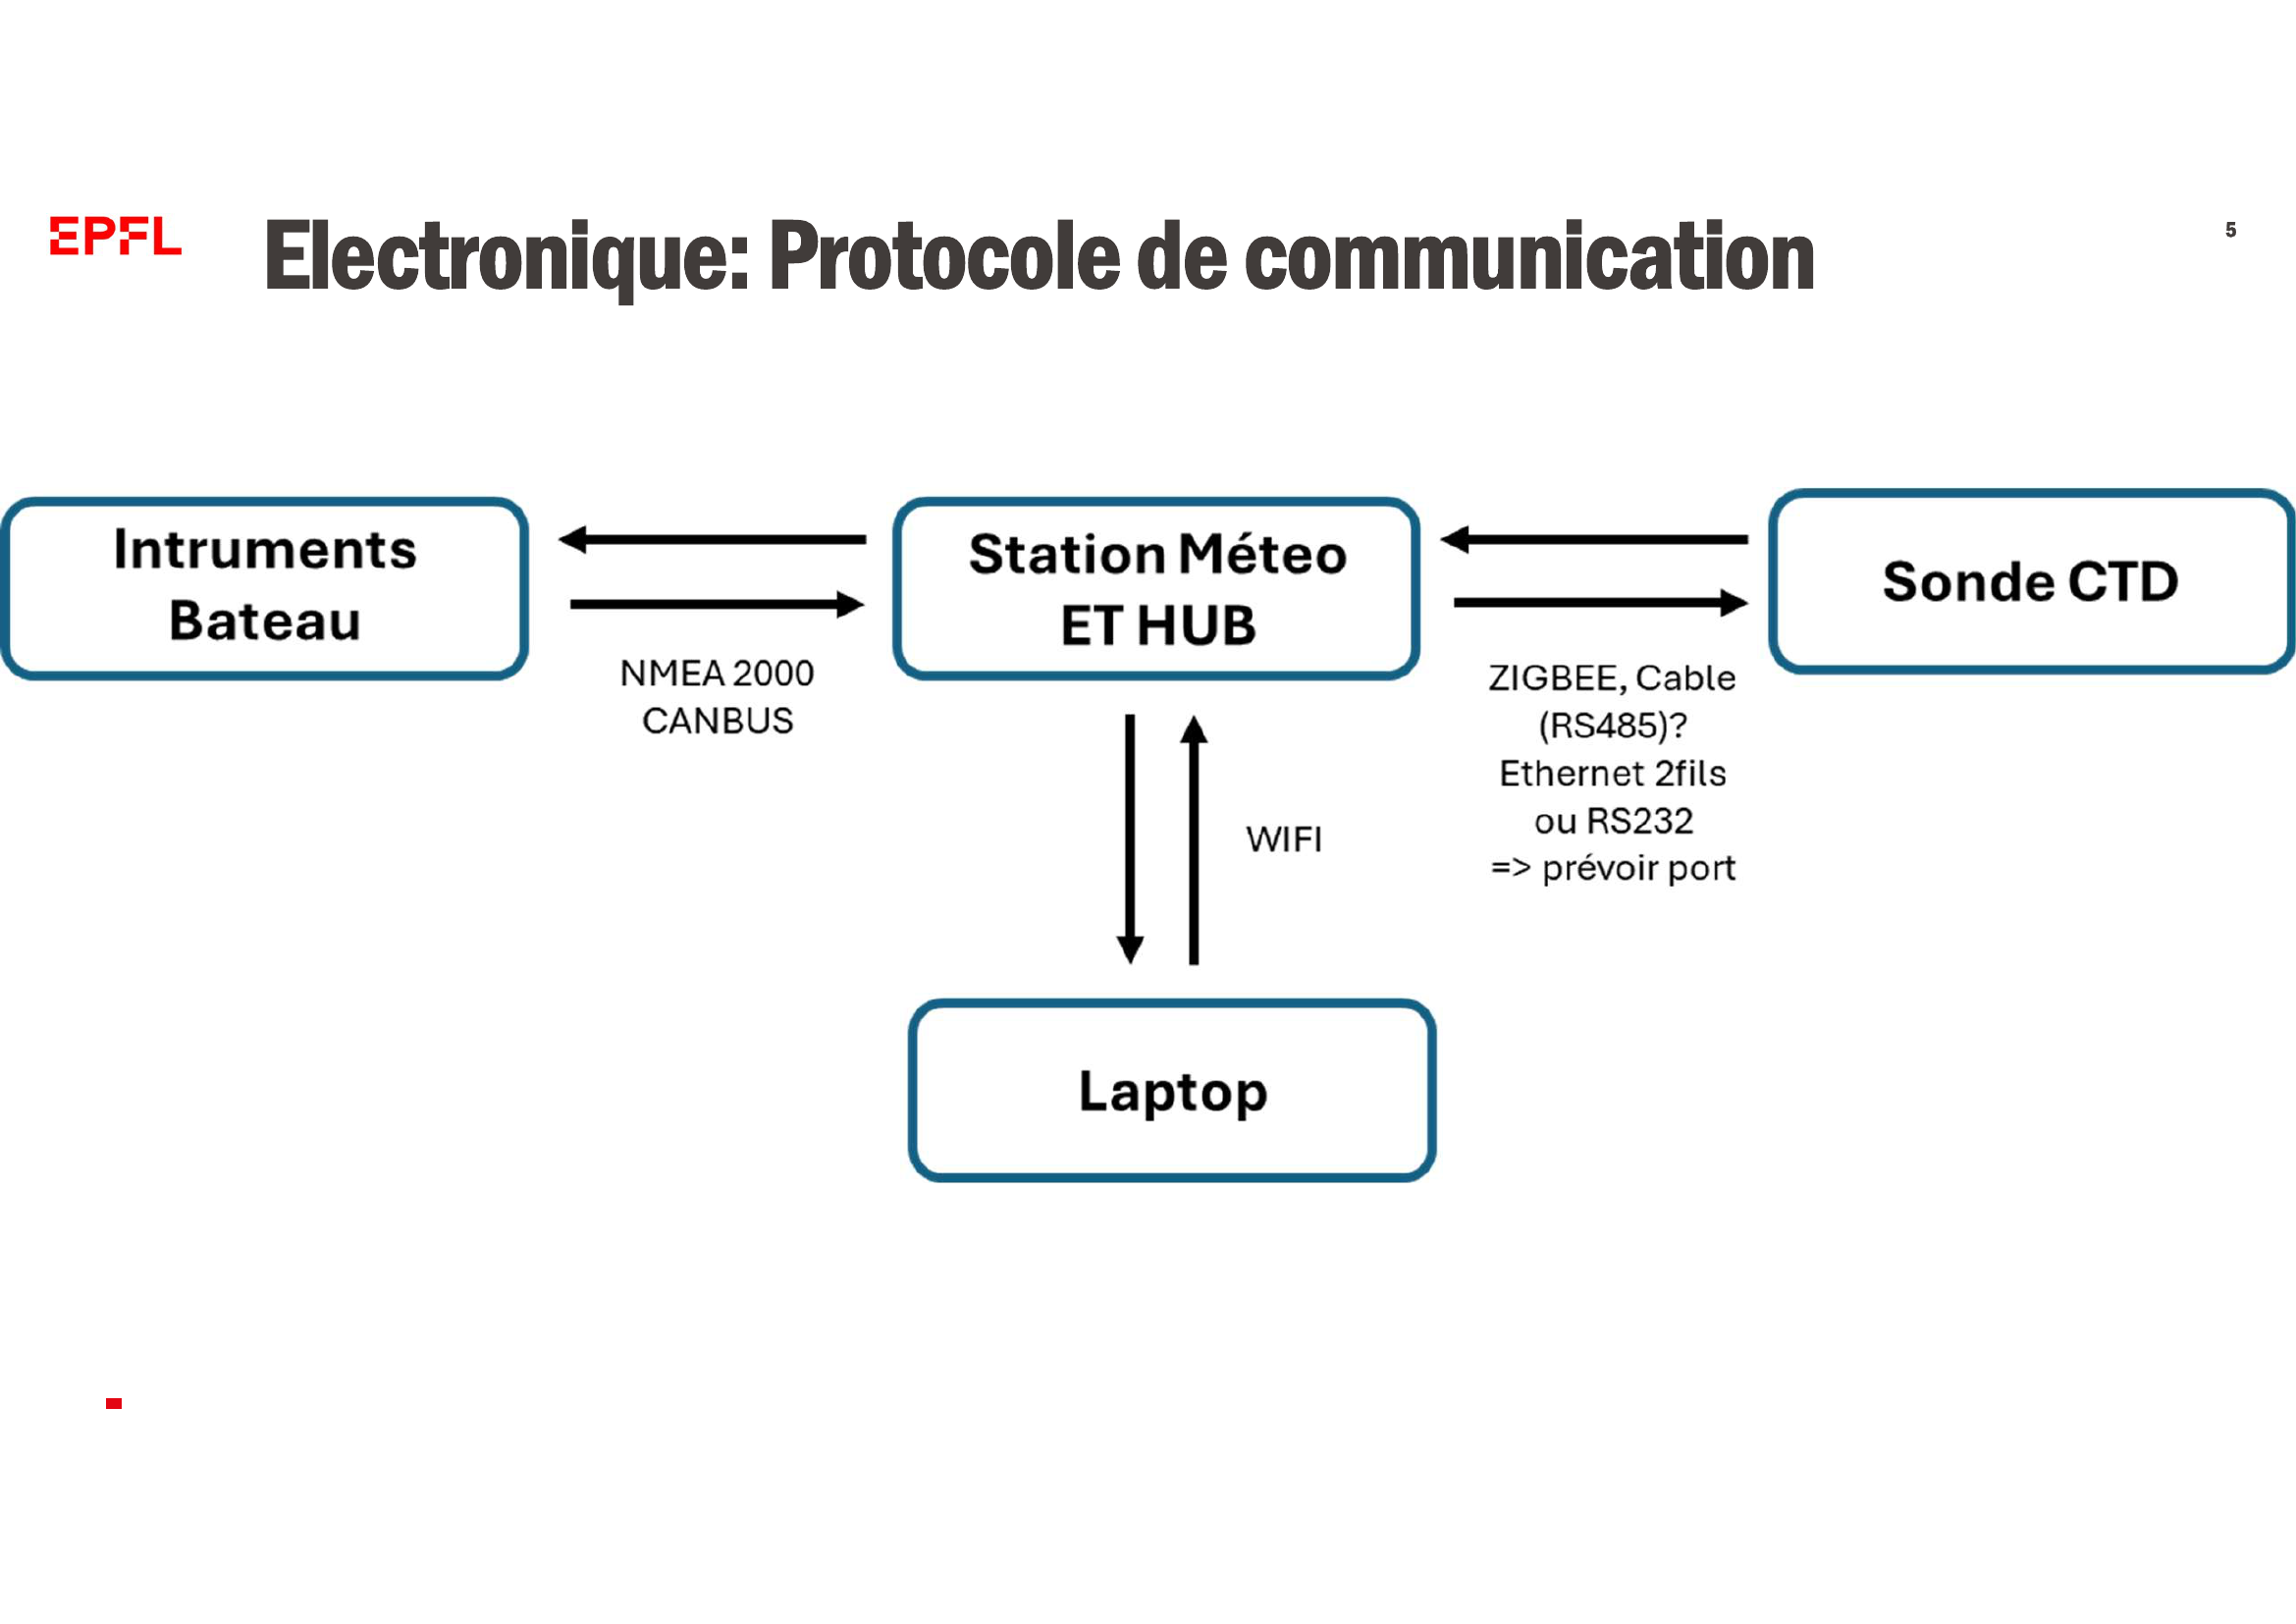
\includegraphics[width=0.85\textwidth]{images/protocole_comm.png}
  \caption{Schéma du protocole de communication entre les différents systèmes.}
  \label{fig:protocole_comm}
\end{figure}

\subsection{PCB étage 1 — Contrôle et connectivité}\label{subsec:pcb1}

Le premier étage regroupe les composants dédiés au traitement central, à la
connectivité réseau et à l'alimentation. La carte est de forme circulaire pour
s'insérer dans le boîtier cylindrique décrit à la section~\ref{sec:mecanique}.
Les composants retenus sont listés dans le tableau~\ref{tab:pcb1}.

\begin{table}[H]
  \centering
  \caption{Composants du PCB étage 1.}
  \label{tab:pcb1}
  \begin{tabular}{llc}
    \toprule
    \textbf{Fonction} & \textbf{Référence} & \textbf{Qté} \\
    \midrule
    Microcontrôleur principal & ESP32 DevKit M V1         & 1 \\
    Module Zigbee             & XIAO ESP32C6              & 1 \\
    Lecteur carte SD          & Adafruit micro SD         & 1 \\
    GPS                       & Adafruit GPS              & 1 \\
    Transceiver CAN           & MCP2515 (NMEA 2000)       & 1 \\
    Convertisseur de niveaux  & Bi-Directional Converter  & 1 \\
    Régulateur DC-DC          & Purecrea LM2596           & 1 \\
    \bottomrule
  \end{tabular}
\end{table}

\paragraph{Microcontrôleur.} L'\textit{ESP32 DevKit M V1} est choisi pour sa
double connectivité Wi-Fi et Bluetooth, sa puissance de calcul (240 MHz, deux
cœurs) et son large écosystème de bibliothèques Arduino/PlatformIO. Il orchestre
la totalité des échanges entre les capteurs, le stockage et la transmission.

\paragraph{Stockage et localisation.} La carte SD (interfacée en SPI) assure
l'enregistrement local des mesures en cas de perte de connexion Wi-Fi. Le module
GPS fournit l'horodatage et la position géographique de chaque mesure, indispensables
pour la corrélation avec d'autres sources de données oceanographiques.

\paragraph{Alimentation.} Le régulateur buck \textit{LM2596} convertit la tension
batterie (typiquement 12 V) en 5 V pour alimenter l'ensemble du système. Le
convertisseur de niveaux logiques bidirectionnel est nécessaire pour l'interfaçage
entre les composants 3,3 V (ESP32) et 5 V (certains capteurs et le transceiver CAN).

\begin{figure}[H]
  \centering
  \begin{subfigure}[b]{0.48\textwidth}
    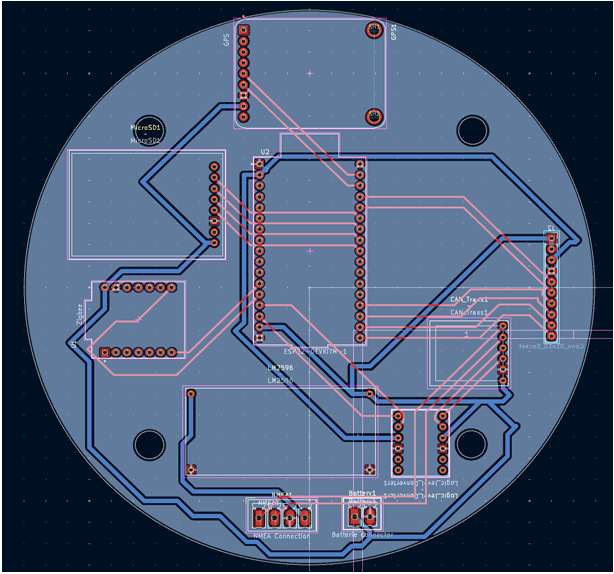
\includegraphics[width=\textwidth]{images/pcb1_routage.png}
    \caption{Routage KiCad}
  \end{subfigure}
  \hfill
  \begin{subfigure}[b]{0.48\textwidth}
    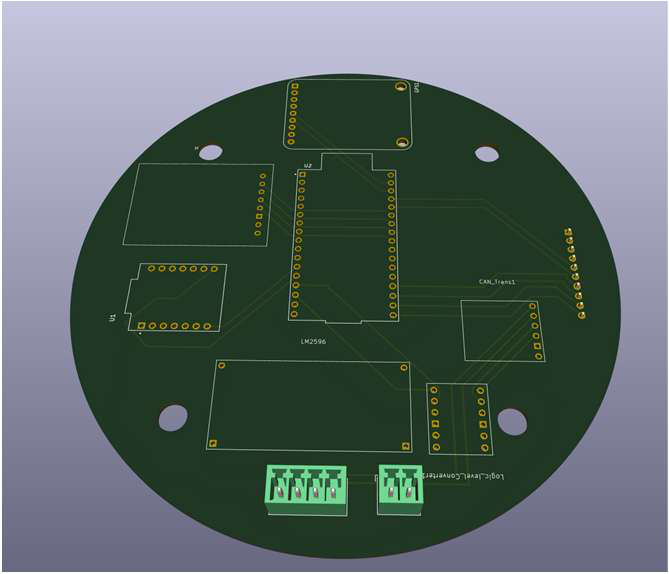
\includegraphics[width=\textwidth]{images/pcb1_3d.png}
    \caption{Rendu 3D}
  \end{subfigure}
  \caption{PCB étage 1 : contrôle et connectivité.}
  \label{fig:pcb1}
\end{figure}

\subsection{PCB étage 2 — Capteurs}\label{subsec:pcb2}

Le deuxième étage regroupe l'ensemble des capteurs environnementaux.
Les composants retenus sont listés dans le tableau~\ref{tab:pcb2}.

\begin{table}[H]
  \centering
  \caption{Composants du PCB étage 2.}
  \label{tab:pcb2}
  \begin{tabular}{llc}
    \toprule
    \textbf{Fonction}                    & \textbf{Référence}        & \textbf{Qté} \\
    \midrule
    Accéléromètre 6 axes                 & Purecrea MPU-6050         & 1 \\
    Température / Pression / Humidité    & BME280                    & 1 \\
    Capteur de lumière                   & BH1750                    & 1 \\
    Caméra                               & Joy-it ESP32 camera board & 1 \\
    Capteur de particules fines          & SPS30 (Sensirion)         & 1 \\
    \bottomrule
  \end{tabular}
\end{table}

\paragraph{Qualité de l'air.} Le capteur \textit{SPS30} de Sensirion mesure la
concentration massique des particules PM$_{1.0}$, PM$_{2.5}$, PM$_4$ et PM$_{10}$
par diffraction laser. Sa précision et sa robustesse en font un standard dans les
réseaux de surveillance de la qualité de l'air.

\paragraph{Météorologie.} Le \textit{BME280} mesure simultanément la température
($\pm 1\,^{\circ}$C), la pression atmosphérique ($\pm 1$\,hPa) et l'humidité
relative ($\pm 3$\,\%). Le \textit{BH1750} fournit une mesure de l'éclairement
lumineux en lux, utilisée comme indicateur d'irradiance solaire.

\paragraph{Orientation.} L'accéléromètre \textit{MPU-6050} (IMU 6 axes : 3 axes
accélération + 3 axes gyroscope) permet de corriger les mesures en fonction de
l'orientation et du tangage/roulis du bateau. Cette correction est essentielle
pour les mesures d'irradiance et pour la segmentation d'images nuageuses.

\paragraph{Vision.} La caméra \textit{Joy-it ESP32} orientée vers le zénith
acquiert des images périodiques du ciel pour l'algorithme de détection de
couverture nuageuse décrit à la section~\ref{sec:vision}.

\begin{figure}[H]
  \centering
  \begin{subfigure}[b]{0.48\textwidth}
    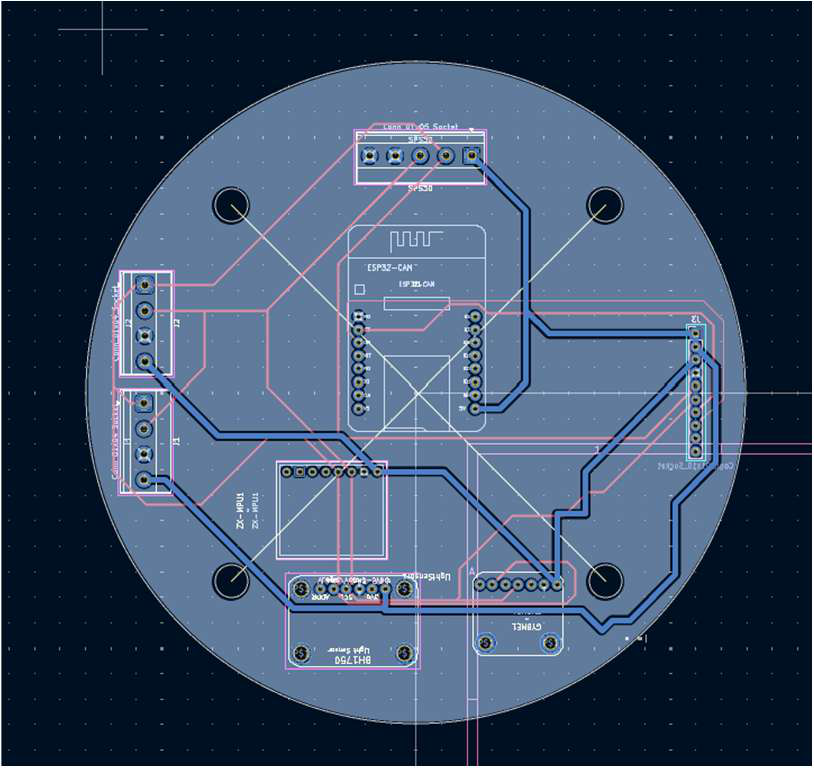
\includegraphics[width=\textwidth]{images/pcb2_routage.png}
    \caption{Routage KiCad}
  \end{subfigure}
  \hfill
  \begin{subfigure}[b]{0.48\textwidth}
    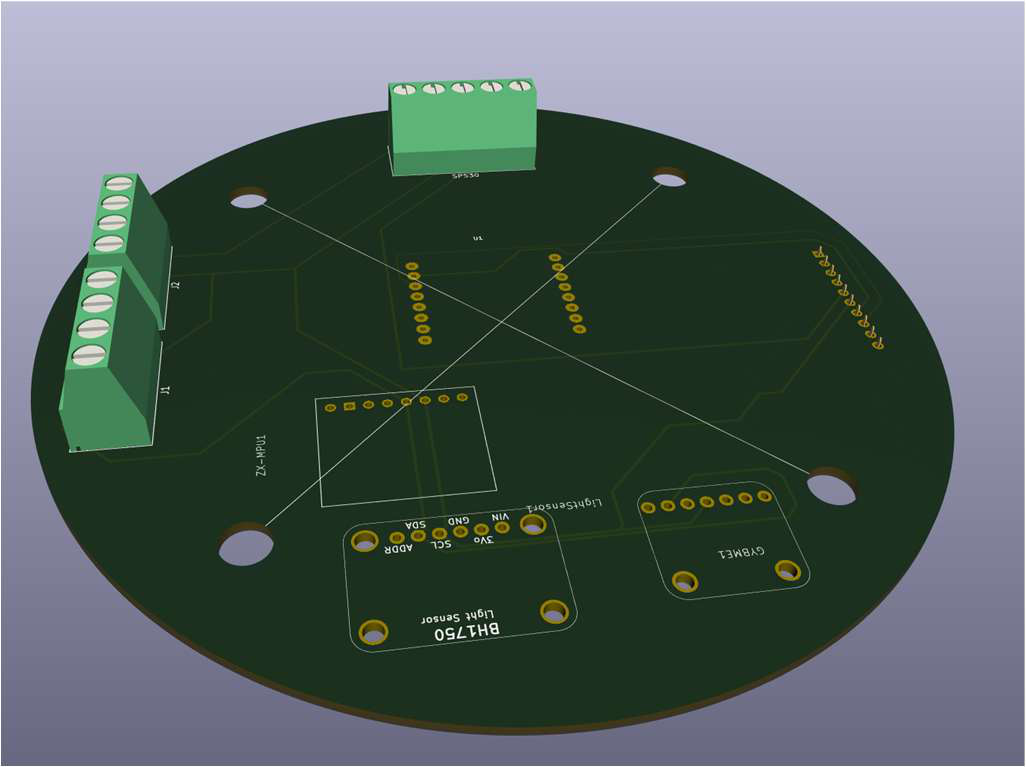
\includegraphics[width=\textwidth]{images/pcb2_3d.png}
    \caption{Rendu 3D}
  \end{subfigure}
  \caption{PCB étage 2 : capteurs environnementaux.}
  \label{fig:pcb2}
\end{figure}

\subsection{Réalisation}\label{subsec:realisation_elec}

L'ensemble des composants électroniques --- capteurs, PCB, câbles et adaptateurs
--- a été réceptionné. Les soudures et l'assemblage électronique ont été réalisés.
Un premier firmware de test a été développé pour valider la communication entre
les différents périphériques et vérifier les lectures des capteurs.
